\chapter{Additional Comments and Results}
\label{ap:appendix}

\section{Least Squares Fit to High Energy Crab Emission}
\label{ap:lsqrs}
In \cref{fig:sed_fit_he} I performed a least-squares fit to flux data for a log-parabolic energy spectrum with
parameters $\alpha$, $\beta$, and the amplitude $A$.
The matrix below shows the covariance of the parameters as estimated by \scipy's \lstinline{curve_fit} method. 
The \scipy method uses the Levenberg-Marquardt~\cite{levenberg} algorithm and estimates the covariance via the Hessian matrix in the minimum. 
The entries on the diagonal show the variance of the corresponding parameter.
\begin{equation*}
    \input{build/sed_fit_he_matrix.txt}
\end{equation*}



\newpage
\section{SSC Fit to Crab Nebula Flux Data}
\label{ap:ssc_fit}
\noindent%
\begin{minipage}{\linewidth}% to keep image and caption on one page
\makebox[\linewidth]{%        to center the image
  \includegraphics{build/naima_corner.pdf}}
\captionof{figure}[Correlation between fit parameters of the \naima SED model.]{This figure shows the correlation between the sampled parameters for figure \ref{fig:ssc_fit}.
The red dots indicate the median. Tick labels on the axis are placed at the 1\th, 99\th and 50\th percentile.
The histograms on the diagonal show the marginalized distributions of the parameters labeled on the lower axis.
Some of these parameters show strong correlations, which need to be taken into account when interpreting the 
errors given in~\ref{tab:ssc_fit_results}\label{fig:ssc_correlation}}%      only if needed  
\end{minipage}
% \begin{figure}
%   \centering
%   \includegraphics[width=\textwidth]{build/naima_corner.pdf}
%   \caption[}
%   \label{fig:ssc_correlation}
% \end{figure}
\begin{table}
  \centering
  \caption[Posterior distributions of the SED model parameters]{List of free parameters for the SSC model fitted to fluxes from the Crab Nebula. The left column shows the median 
  sample values with their 16\th and 84\th percentiles. The center columns shows the parameter values for all sampled chains 
  in gray and the median value of all chains in red. The rightmost column shows the marginalized posterior distribution 
  of each parameter. The shaded gray area indicates the 16\th and 84\th percentiles.}
  \label{tab:ssc_fit_results}
  \setlength\tabcolsep{0pt}
  \begin{tabular*}{\textwidth}{l@{\extracolsep{\fill}}c@{\hskip 1.5\tabcolsep}c}
    \textbf{Parameter}  & \textbf{Chain} & \textbf{Distribution}\\
    % \hline
      \input{build/naima_results/param_0.txt}&
      \raisebox{-0.5\totalheight}{\includegraphics{build/naima_results/chain_0.pdf}} &
      \raisebox{-0.5\totalheight}{\includegraphics{build/naima_results/density_0.pdf}} \\
      \input{build/naima_results/param_1.txt}&
      \raisebox{-0.5\totalheight}{\includegraphics{build/naima_results/chain_1.pdf}} &
      \raisebox{-0.5\totalheight}{\includegraphics{build/naima_results/density_1.pdf}} \\
      \input{build/naima_results/param_2.txt}&
      \raisebox{-0.5\totalheight}{\includegraphics{build/naima_results/chain_2.pdf}} &
      \raisebox{-0.5\totalheight}{\includegraphics{build/naima_results/density_2.pdf}} \\
      \input{build/naima_results/param_3.txt}&
      \raisebox{-0.5\totalheight}{\includegraphics{build/naima_results/chain_3.pdf}} &
      \raisebox{-0.5\totalheight}{\includegraphics{build/naima_results/density_3.pdf}} \\
      \input{build/naima_results/param_4.txt}&
      \raisebox{-0.5\totalheight}{\includegraphics{build/naima_results/chain_4.pdf}} &
      \raisebox{-0.5\totalheight}{\includegraphics{build/naima_results/density_4.pdf}} \\
      \input{build/naima_results/param_5.txt}&
      \raisebox{-0.5\totalheight}{\includegraphics{build/naima_results/chain_5.pdf}} &
      \raisebox{-0.5\totalheight}{\includegraphics{build/naima_results/density_5.pdf}} \\
  \end{tabular*}
\end{table}




\section{Historical Evidence of Crab Supernova}
\label{ap:crab}
Chinese records provide relatively reliable 
descriptions of variable phenomena in the sky. Ancient Chinese astronomers speak of \enquote{Guest Stars} 
whenever such a variable star was observed. Compared to European records, these document are relatively reliable. 
The earliest records of Guest Stars in Chineses history date back to the Han dynasty approximately 200 B.C.~\cite{chinese_astro}

The figure below shows the only known historical mention of the supernova that is now the Crab Nebula. 
A Chinese astronomer recorded the phenomenon in a letter to his emperor.
The dates and description match that of a supernova consistent with the 
location of the Crab Nebula.

% \noindent%
% \begin{minipage}{\linewidth}% to keep image and caption on one page
%   \makebox[\linewidth]{%        to center the image
%   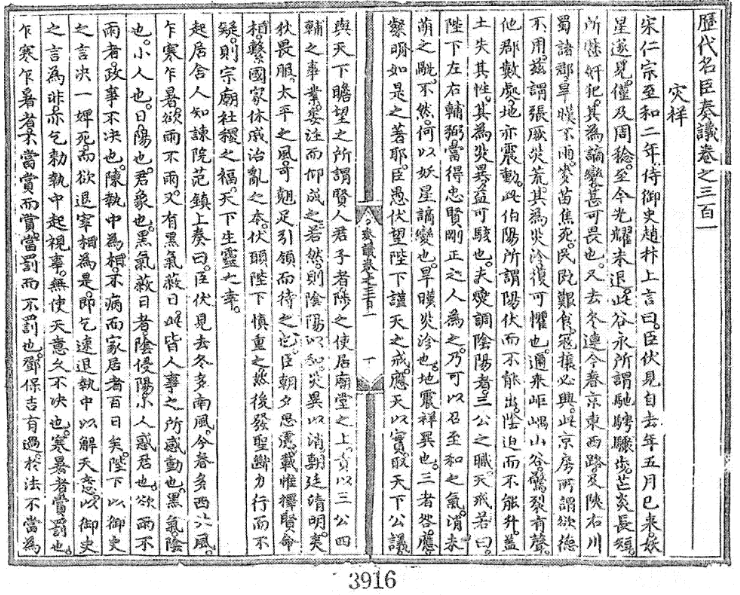
\includegraphics[width=0.8\textwidth]{figures/sn1054_chinese.png}}%
%   \captionof{figure}[Historical Chinese records about the Crab supernova]{Chinese records of the Lidai Mingchen Zouyi~\cite[535]{chinese_history}, which dates to 1414. The passage about the Crab Nebula supernova (SN 1054)
%   as was translated in \cite{crab_chinese}. 
%   The passage reads: \enquote{2\nd year of the Zhihe reign period of Emperor Renzong of 
%   Song [1055]; Attendant Censor Zhao Bian submitted a letter saying: \enquote{Your servant considers that, since the 5th month of last
%   year [when] the baleful star appeared, a full year has passed and until now its brilliance has not faded [lit. 'retreated']}. 
%   This is what Gu Yong meant by \enquote{its rapid movement, the variations in the length of its flaming rays, and the [asterisms] on which
%   it has trespassed successively}, as a censorious anomaly it is greatly to be feared.}.\label{fig:crab_chinese}}%
% \end{minipage}%
\begin{figure}[h]
  \centering
  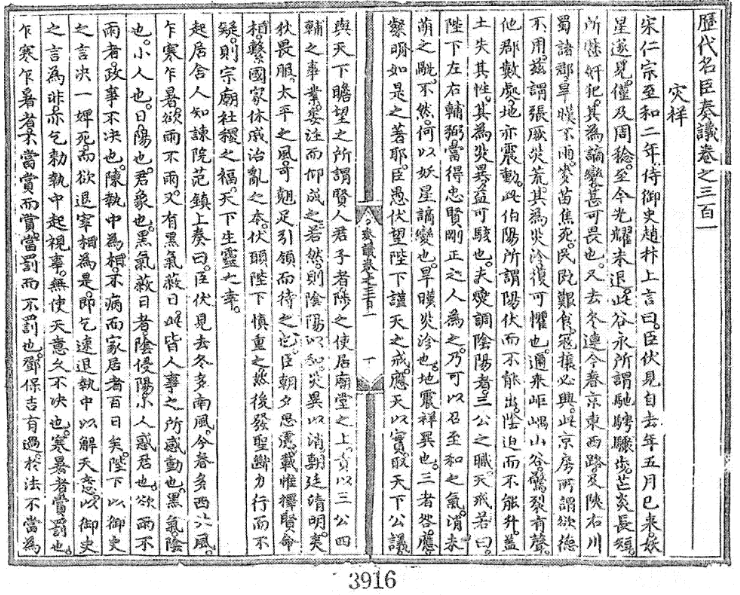
\includegraphics[width=0.8\textwidth]{figures/sn1054_chinese.png}
  % (\fontspec{Heiti SC Light}{歷代名臣奏議})
  \caption[Historical Chinese records about the Crab supernova]{Chinese records of the Lidai Mingchen Zouyi~\cite[535]{chinese_history}, which dates to 1414.
    The passage about the Crab Nebula supernova (SN 1054)as translated in \cite{crab_chinese}. 
    The passage reads: \enquote{2\nd year of the Zhihe reign period of Emperor Renzong of 
    Song [1055]; Attendant Censor Zhao Bian submitted a letter saying: \enquote{Your servant considers that, since the 5th month of last
    year [when] the baleful star appeared, a full year has passed and until now its brilliance has not faded [lit. 'retreated']}. 
    This is what Gu Yong meant by \enquote{its rapid movement, the variations in the length of its flaming rays, and the [asterisms] on which
    it has trespassed successively}, as a censorious anomaly it is greatly to be feared.}.
    }\label{fig:crab_chinese}
\end{figure}


\section{Profile Likelihood Solution}
\label{ap:wstat}
The full Poisson likelihood includes a nuisance parameter for each energy bin that describes the number of background counts.
These nuisance parameters can be removed by \enquote{profiling} the likelihood.
Solving \eqref{eq:ll_profile} for $\mu_b$ yields
\begin{equation}
  \mu_b =\frac{N_{\mathrm{off}}\alpha + N_{\mathrm{on}}\alpha - \alpha\mu_s - \mu_s - \sqrt{K}}{2\alpha(\alpha + 1)}
\end{equation}
where
\begin{equation*}
  K = \alpha^2 (N_{\mathrm{off}}^2 +  2 N_{\mathrm{off}} (N_{\mathrm{on}} + \mu_s) + N_{\mathrm{on}}^2 - 2 N_{\mathrm{on}} \mu_s + \mu_s^2) + 2 \alpha \mu_s ((N_{\mathrm{off}} - N_{\mathrm{on}}) + \mu_s) + \mu_s^2.
\end{equation*}
This expression can be substituted into \eqref{eq:full_ll} resulting in the profile likelihood which has no dependence on $\mu_b$ anymore.
Special care has to be taken when implementing this formula for zero counts in the data. 
See \url{https://docs.gammapy.org/0.11/stats/fit_statistics.html} for some information about edge cases.


\newpage
\section{Implementation for \pymc and \theano}
\label{ap:sampler_details}
The higher the sampling rate, the quicker the fit. Spending some time to optimize the code to integrate the spectral model brings a large speed improvement.
The listing below shows how the trapezoidal operation is implemented in a vectorized way using the \numpy~\cite{numpy} library.

\begin{minipage}{\textwidth}
\begin{mdframed}[backgroundcolor=white!20!black,leftmargin=0cm,rightmargin=0cm, skipabove=0pt, innerleftmargin=0,innerrightmargin=0,]
\begin{pythonlst}[basicstyle=\lstsansserif]
  # Define x and delta x. This can be pre-computed once.
  d = np.tile(np.linspace(0, 1, num=num_nodes), num_bins).reshape(num_bins, -1) 
  xs = (d * bin_widths[:, None]) + bin_edges[0:-1, None] 
  delta_xs = np.diff(xs)

  # Compute the integral of f using theano's symbolic sum operation. 
  y = f(xs, parameters)
  integral = 0.5 * theano.tensor.sum((y[:, 0:-1] + y[:, 1:]) * delta_xs, axis=1) 
\end{pythonlst}
\end{mdframed}
\end{minipage}

This unassuming piece of code brings a dramatic speed increase of at least a factor of 10. 
Instead of building single scalar gradients for each energy bin, \theano can build the Jacobian for a single tensor object. 
The gradient of the integral with respect to the parameters $N_0, \alpha, \beta$ can be build automatically. The \pymc model seems to 
sample faster when the gradients are precomputed.
Since the integral limits are constant, we can apply Leibniz integral rule~\cite{leibniz_rule} and switch the order of the differential and the integration
\begin{align*}
  \dddp{c}{\alpha} &= \ddp{\alpha} \int\limits_{\Delta \etrue} N(E; N_0, \alpha, \beta) \diff{E} = \int\limits_{\Delta \etrue} \ddp{\alpha} N(E; N_0, \alpha, \beta) \diff{E} \\
  &= \int\limits_{\Delta \etrue} \ddp{\alpha} N_0 \biggl( \frac{E}{E_0} \biggr)^{-\alpha -\beta \log_{10}\left(\frac{E}{E_0}\right)} \diff{E} \\
  &= -N_0 \int\limits_{\Delta \etrue} \biggl(\frac{E}{E_0} \biggr)^{-\alpha -\beta \log_{10}\bigl(\frac{E}{E_0}\bigr)} \log\biggl(\frac{E}{E_0}\biggr) \diff{E}.
\end{align*}
Equivalently for $\beta$
\begin{equation*}
  \dddp{c}{\beta} = -\int\limits_{\Delta \etrue} \frac{1}{\log(10)} \log^2\left(\frac{E}{E_0}\right) \biggl( \frac{E}{E_0} \biggr)^{-\alpha -\beta \log_{10}\left(\frac{E}{E_0}\right)}  \diff{E}
\end{equation*}
and last but not least the amplitude parameter $N_0$
\begin{equation*}
  \dddp{c}{N_0} =  \int\limits_{\Delta \etrue} \biggl( \frac{E}{E_0} \biggr)^{-\alpha -\beta \log_{10}\left(\frac{E}{E_0}\right)} \diff{E}.
\end{equation*}
The \pymc model can now be sampled at a rate of several hundred samples per second. The listing below shows the definition of the \pymc model.
The full code can be accessed at \github{tudo-astroparticlephysics/ll_experiments}.

\begin{minipage}{\textwidth}
  \begin{mdframed}[backgroundcolor=white!20!black,leftmargin=0cm,rightmargin=0cm, skipabove=0pt, innerleftmargin=0,innerrightmargin=0,]
  \begin{pythonlst}
  amplitude = pm.HalfFlat('amplitude')
  alpha = pm.HalfFlat('alpha')
  beta = pm.HalfFlat('beta')

  mu_s = forward_fold_log_parabola(integrator, amplitude, alpha, beta, observations)
  mu_b = pm.TruncatedNormal(
      'mu_b',
      lower=0,
      shape=len(off_data),
      mu=off_data,
      sd=5
  )

  pm.Poisson('background', mu=mu_b, observed=off_data, shape=len(off_data))
  pm.Poisson(
    'signal',
     mu=mu_s + exposure_ratio * mu_b,
     observed=on_data,
     shape=len(on_data)
  )
  \end{pythonlst}
  \end{mdframed}
\end{minipage}

\section{Sensitivity and Effective Area for Fixed On Region}
\label[app]{ap:fixed}
The sensitivity curve~\ref{fig:sensitivity} and the effective area plot~\ref{fig:eff_area_optimized} were calculated on an optimized subset of the data. 
Combinations of prediction threshold, multiplicity, and on-region radius were tested to find the best sensitivity.
This might introduce biases and \emph{over-fitting} effects since no independent test data is available. 
To mitigate the effects to some degree, the size of the on-region, $\theta$, is defined in terms of angular resolution. 
This reduces the dimension of the optimization problem and increases runtime drastically.
\begin{figure}
  \centering
  \includegraphics[width=\textwidth]{build/effective_area_optimized_fixed_theta.pdf}
  \caption[Effective area for fixed values of $\theta$]{  
    Effective area for optimized event selection in multiplicity and prediction threshold. The on-region radius $\theta$ was fixed to 
    \SI{50}{\percent} containment of the angular distance between true and estimated position in each energy bin. 
    In comparison to the results shown in \cref{fig:eff_area_optimized}, the values match the reference curve better.
  }
  \label{fig:eff_area_fixed}
  \vspace*{\floatsep}% https://tex.stackexchange.com/q/26521/5764
  \includegraphics[width=\textwidth]{build/sensitivity_fixed.pdf}
  \caption[Sensitivity curve for fixed values of $\theta$]{  
    Sensitivity curve for optimized event selection in multiplicity and prediction threshold. The on-region radius $\theta$ was fixed to 
    \SI{50}{\percent} containment of the angular distance between true and estimated position in each energy bin. 
    The results are slightly worse than the ones shown in \cref{fig:sensitivity}, but still well within the expected performance range.
  }
  \label{fig:sensitivity_fixed}
\end{figure}


\section{Dependency Graph}
The \cref{fig:dep_graph} below shows the dependency of this document. It was created from the Makefile 
by the tool \texttt{makefile2graph}\footnote{\url{https://github.com/lindenb/makefile2graph}} written by Pierre Lindenbaum. 
The output was processed with the \texttt{Gephi}~\cite{gephi} software. \texttt{Gephi} is a graphical user interface to 
modify graphs for visualization. It supports various layout algorithms and search queries in large graphs.
The figure below represents only a part of the dependency graph as one of the nodes calls into yet another Makefile recursively.
Still, the figure summarizes most data dependencies needed for a proper CTA analysis. Managing this complicated construction by hand 
would be a herculean task. I urge anyone performing data analysis of any kind to use a workflow automation tool like \make or \snakemake.

\noindent%
\begin{minipage}{\linewidth}% to keep image and caption on one page
\makebox[\linewidth]{%        to center the image
  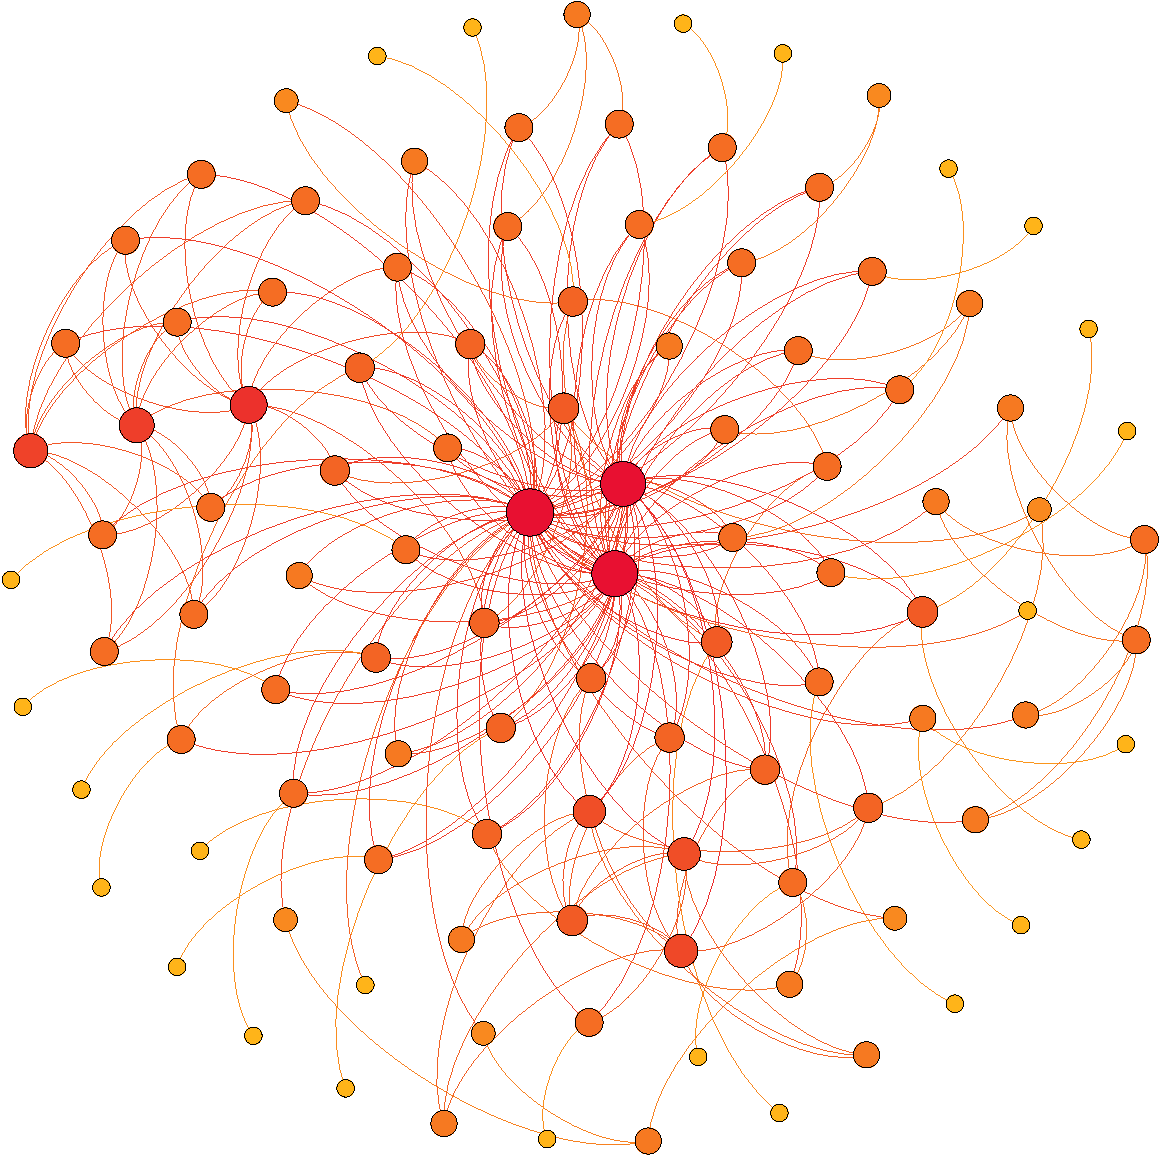
\includegraphics[width=0.6\textwidth]{figures/make_graph.pdf}}
\captionof{figure}[Dependency Graph]{The dependency graph of this document as seen by \make. The inner nodes correspond to the final targets. 
The final pdf file, which is this very document, has the largest degree of all nodes in this graph. Unfortunately, this figure itself cannot 
be created without human interaction and cannot be created fully automatically.  
\label{fig:dep_graph}}%      only if needed  
\end{minipage}


\chapter{Configuration Files}
\label{ap:config}

\section{Configuration for the \aicttools}
\label{ap:aict_config}

The listing below shows the contents of the configuration file used for the \aicttools.
I'd like to take this opportunity and apologize for the terrible name of the \aicttools project.  
I was put on the spot by an approaching deadline and the creative fumes of the day were eluding me. 

\begin{spacing}{0.5}
  \lstinputlisting[basicstyle=\tiny\lstsansserif, multicols=2, language=yaml]{./configs/aict/iact_config.yaml}
\end{spacing}

\section{\python Requirements}
\label{sec:requirements}
I relied heavily on open-source software for every step presented in this thesis.
The most important libraries are listed below in no particular order.
\begin{itemize}
  \item \astropy~\cite{astropy_2013,astropy_2018}
  \item \numpy~\cite{numpy}
  \item \pandas~\cite{pandas}
  \item \sklearn~\cite{sklearn}
  \item \matplotlib~\cite{matplotlib}
  \item \scipy~\cite{scipy}
\end{itemize}

This document itself was built with MacTex-2018 on both macOS Mojave and macOS High Sierra.
% I did not test this on either Windows or Linux 
% \enquote{it should work}.
%  However the listing below shows the required \python packages
The listing below shows all the \python packages and their version numbers which were used to produce the results shown in this document.
given that the \python installation is properly set
\begin{spacing}{0.5}
  \lstinputlisting[basicstyle=\tiny\lstsansserif, multicols=2, language=yaml]{./build/requirements.txt}
\end{spacing}

\section{Configuration for Preprocessing}
\label{ap:preprocess_config}

The listing below shows the contents of the configuration file used for the preprocessing 
of the simulated CTA data. The list of telescope IDs selects the telescopes belonging to 
the so-called HB9 layout of the southern CTA site.

\begin{spacing}{0.6}
  \lstinputlisting[basicstyle=\footnotesize\lstsansserif, language=yaml]{./configs/preprocessing/config.yaml}
\end{spacing}